\documentclass{beamer}
\usepackage[czech]{babel}
\usepackage[utf8]{inputenc}
\usepackage{listings}
\usepackage{graphicx}
\usepackage{tikz}



\title[]{Tvorba aplikace pro simulaci problémů v databázovém systému}


\author[] {Lukáš Hanusek}
\date{27. května 2019}

\mode<presentation>
{
  \usetheme{Frankfurt}
  \usecolortheme{default} 
}



\begin{document}

\begin{frame}
  \titlepage
\end{frame}



\begin{frame}
\frametitle{Požadavky na aplikaci}
\textbf{Aplikace pro hromadné vytěžování několika databázových serverů}

\begin{itemize}
\item Možnost připravit seznam databázových serverů
\item Možnost otestovat dostupnost zadaných databázových serverů
\item Možnost předpřipravit posloupnost SQL příkazů
\item Validace SQL
\item Podpora Oracle Databáze a MS SQL Serveru
\end{itemize}

\end{frame}





\begin{frame}
  \frametitle{Použité technologie pro implementaci aplikace}
  
  \begin{itemize}
      \item Jazyk Java
      \item JDBC
      \item XML pro datové soubory a JAXB
      \item JavaFX
   \end{itemize}
\end{frame}

\begin{frame}
  \frametitle{Struktura aplikace}
      \begin{figure}[h]
  \centering
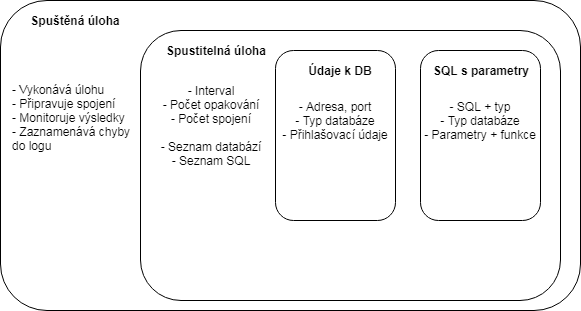
\includegraphics[width=1.0\textwidth]{img/struct.png}
\end{figure}

\end{frame}

\begin{frame}
  \frametitle{Modulární podpora databázových systémů}
  
    \begin{figure}[h]
  \centering
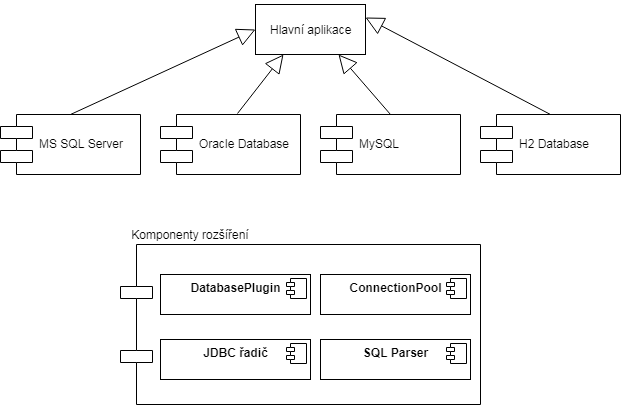
\includegraphics[width=1.0\textwidth]{img/plugins.png}
\end{figure}
\end{frame}



\begin{frame}
  \frametitle{Uživatelské rozhraní - okno editoru}
  \begin{figure}[h]
  \centering
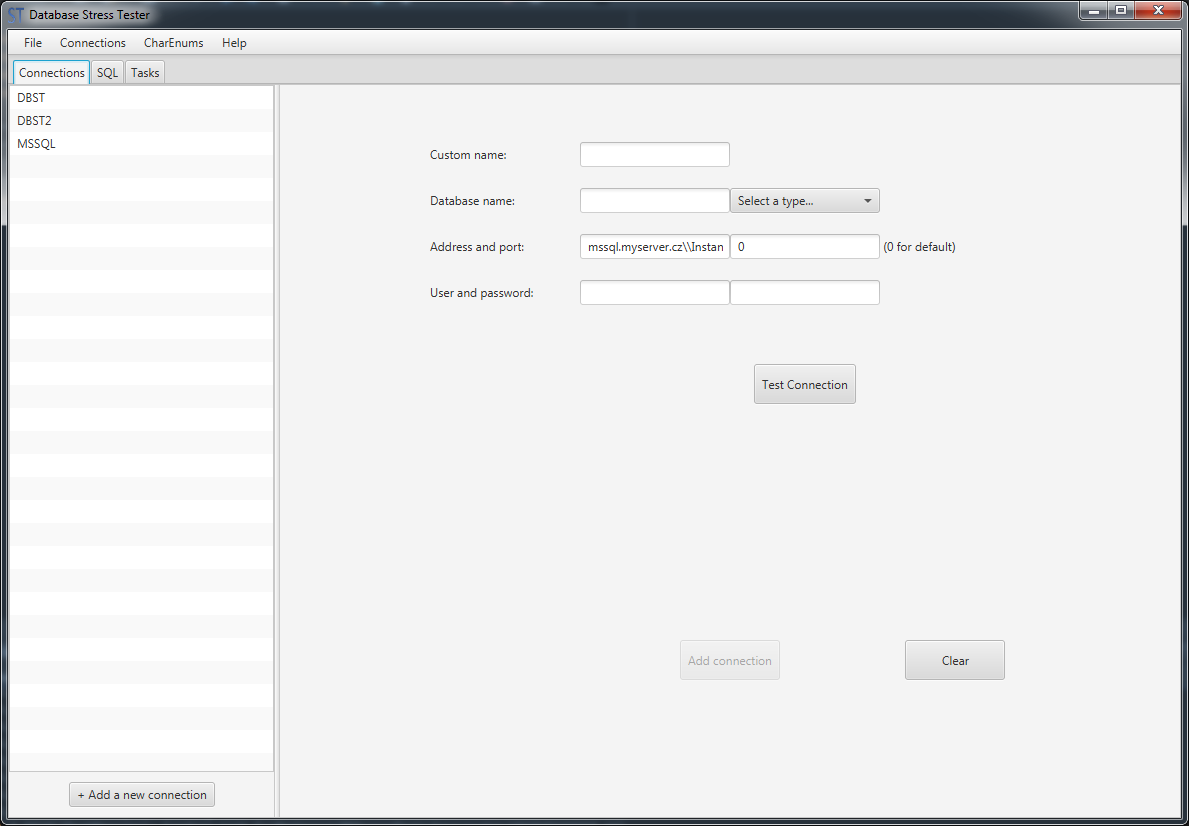
\includegraphics[width=1.0\textwidth]{img/coneditor.png}
\end{figure}

\end{frame}


\begin{frame}
  \frametitle{Uživatelské rozhraní - okno editoru}
  \begin{figure}[h]
\centering
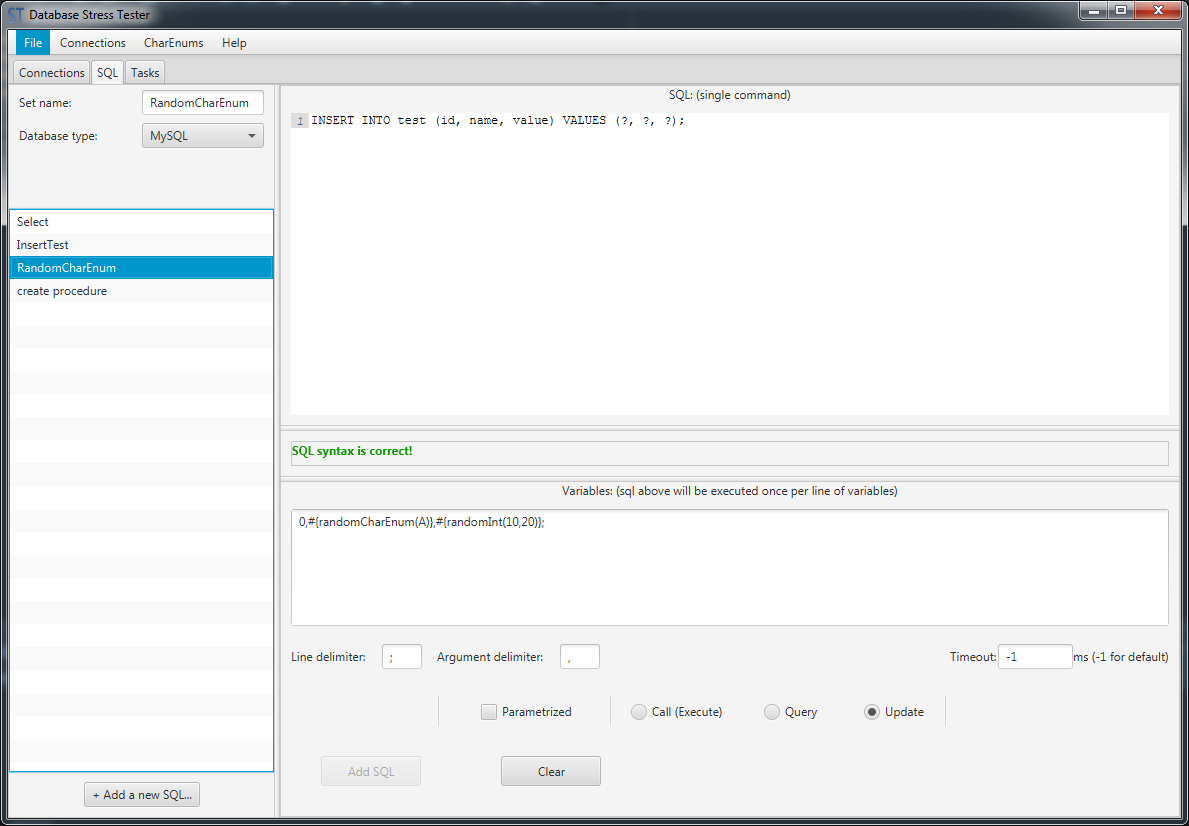
\includegraphics[width=1.0\textwidth]{img/sqleditor.png}
\end{figure}

\end{frame}


\begin{frame}
  \frametitle{Uživatelské rozhraní - okno editoru}
  \begin{figure}[h]
\centering
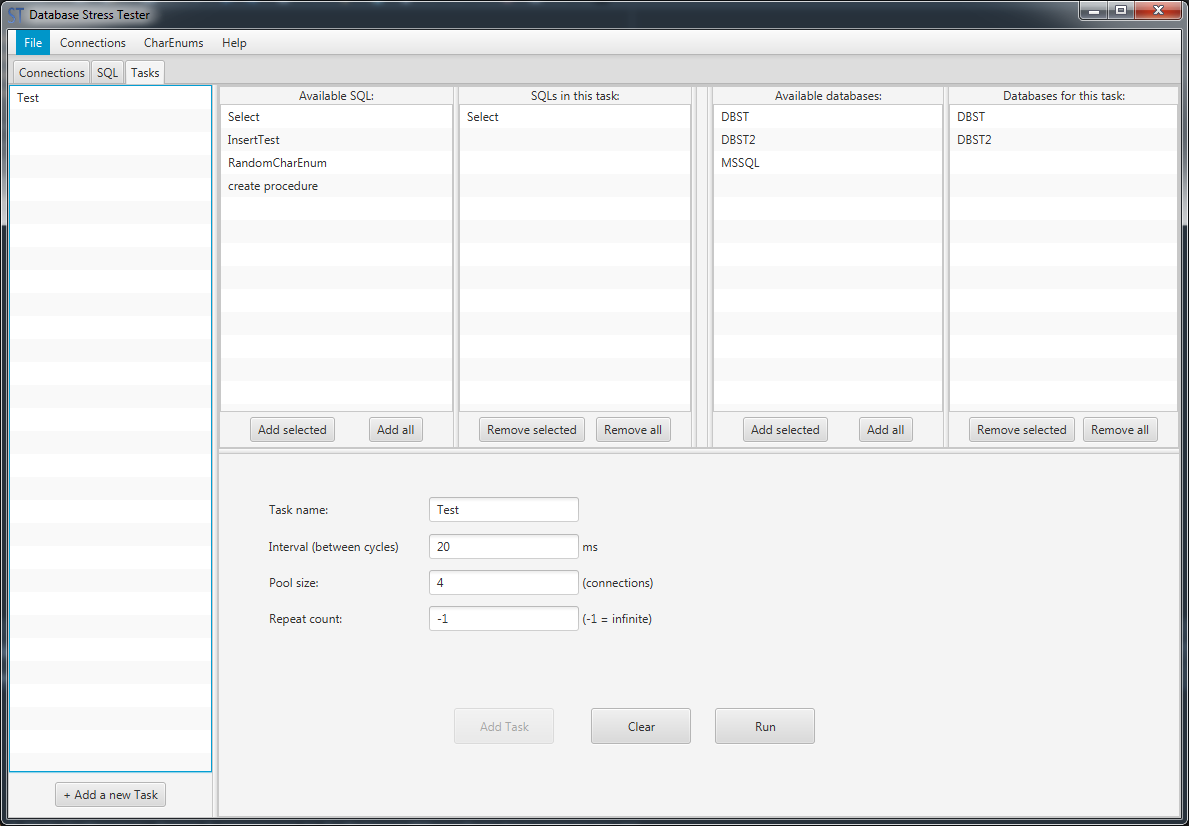
\includegraphics[width=1.0\textwidth]{img/taskeditor.png}
\end{figure}

\end{frame}


\begin{frame}
  \frametitle{Uživatelské rozhraní - okno monitoru}
  \begin{figure}[h]
\centering
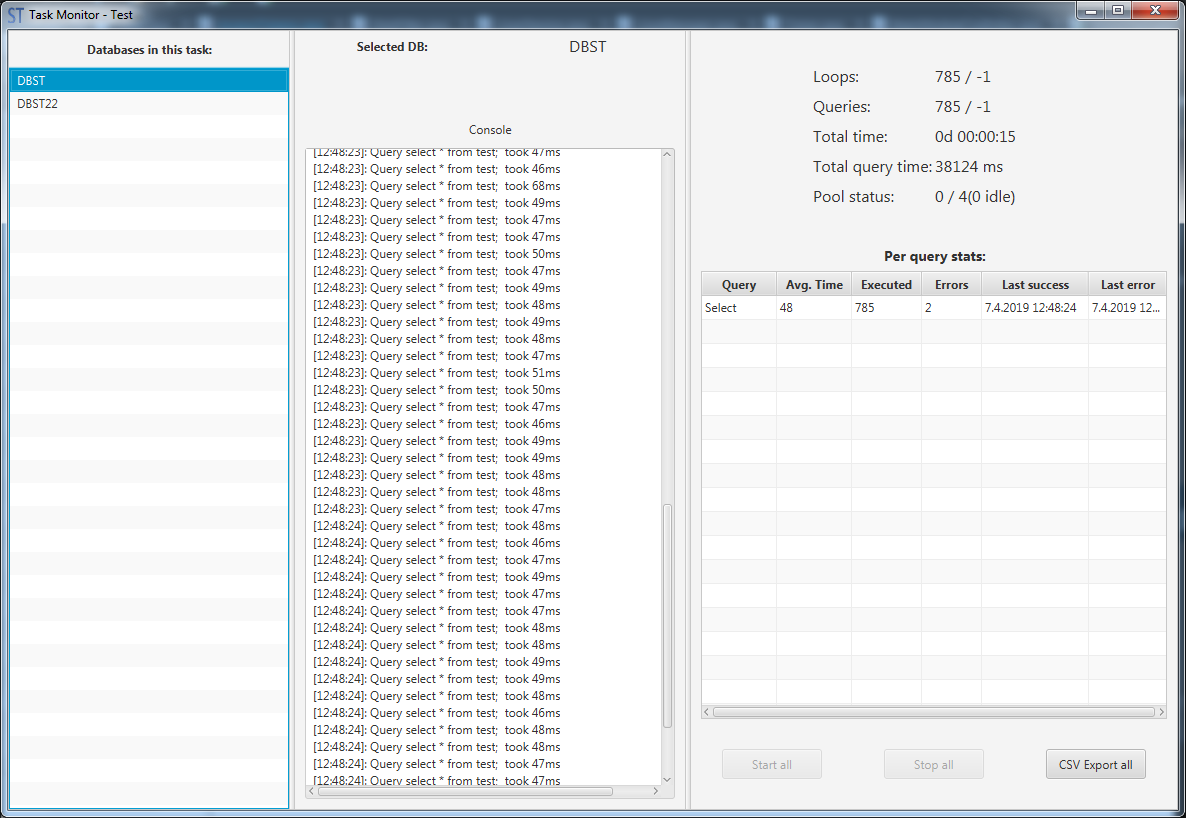
\includegraphics[width=1.0\textwidth]{img/taskmonitor.png}
\end{figure}

\end{frame}




\begin{frame}
  \frametitle{Uživatelem definované funkce}
    \begin{figure}[h]
  \centering
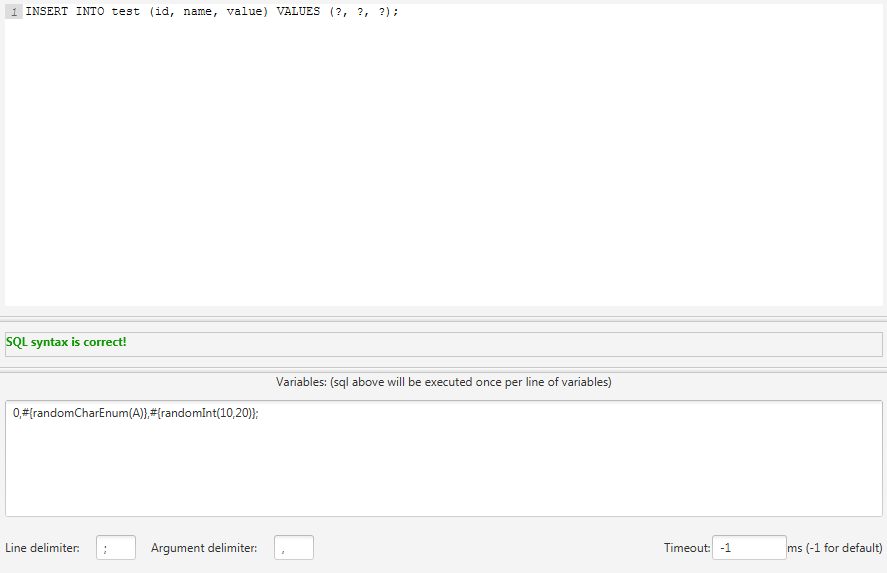
\includegraphics[width=1.0\textwidth]{img/function.png}
\end{figure}
\end{frame}



\begin{frame}
  \frametitle{Uživatelem definované funkce}
  \begin{itemize}
\item 
\textit{Funkce} \textbf{randomInt(MIN,MAX)}:\newline
\textit{Argumenty:}\newline
MIN - definuje minimální velikost generovaného čísla\newline
MAX - definuje maximální velikost generovaného čísla\newline

\textit{Příklad použití funkce:}\newline
\#\{randomInt(1,10)\} - náhodné číslo v rozsahu 1 až 10

\item
\textit{Funkce} \textbf{randomCharEnum(enum)}:\newline
\textit{Argumenty:}\newline
enum - jméno posloupnosti znaků, která bude použita pro generování nové náhodné posloupnosti\newline

\textit{Příklad použití funkce:}\newline
\#\{randomCharEnum(A)\} - vygeneruje náhodnou posloupnost znaků z posloupnosti se jménem '\textit{A}'

\end{itemize}
\end{frame}



\begin{frame}
  \frametitle{SQL Parser}
\begin{table}[!htbp]
	\small{\textbf{ANTLR}: SELECT * FROM TEST}
	\vskip 0.1cm
	\begin{tabular}{llll}
		\hline
		Parser & První spuštění & Opakované spuštění\\
		\hline
		PL-SQL & 1831 ms & 2 ms  \\
        T-SQL & 525 ms & 1 ms  \\
        MySQL & 428 ms & 1 ms  \\
		\hline
	\end{tabular}
\end{table}

\begin{table}[!htbp]
	\small{\textbf{JSql}: SELECT * FROM TEST}
	\vskip 0.1cm
	\begin{tabular}{llll}
		\hline
		Parser & První spuštění & Opakované spuštění\\
		\hline
		Jsql & 30 ms & 0.26 ms \\
		\hline
	\end{tabular}
\end{table}

\end{frame}



\begin{frame}
  \frametitle{SQL Parser}

\begin{table}[!htbp]
	\small{\textbf{ANTLR}: SELECT COUNT(*) FROM TEST WHERE CID = 5 AND PRICE \textless  100 GROUP BY NAME ORDER BY PRICE}
	\vskip 0.1cm
	\begin{tabular}{llll}
		\hline
		Parser & První spuštění & Opakované spuštění\\
		\hline
		PL-SQL & 2522 ms & 6 ms  \\
        T-SQL & 479 ms & 6 ms  \\
        MySQL & 364 ms & 5 ms \\
		\hline
	\end{tabular}
\end{table}



\begin{table}[!htbp]
	\small{\textbf{JSql}: SELECT COUNT(*) FROM TEST WHERE CID = 5 AND PRICE \textless  100 GROUP BY NAME ORDER BY PRICE}
	\vskip 0.1cm
	\begin{tabular}{llll}
		\hline
		Parser & První spuštění & Opakované spuštění\\
		\hline
		Jsql & 33 ms & 0.75 ms\\
		\hline
	\end{tabular}
\end{table}


\end{frame}


\begin{frame}
\frametitle{Závěr}
    \begin{figure}[h]
  \centering
  Děkuji za pozornost.
  \vskip 3cm
  Lukáš Hanusek
\end{figure}
\end{frame}







\end{document}